Im Rahmen der vorliegenden Arbeit konnte die Funktionalität des Moduls \texttt{mpshift} deutlich erweitert werden. Durch die Implementierung des \acf{cosmo} besteht nun die Möglichkeit Umgebungseffekte bei der Berechnung von chemischen Abschirmungskonstanten mit einzubeziehen. Zusätzlich ermöglicht dieses Modell die Kompensation von Gegenladungen, was insbesondere für hoch geladene anionische Verbindungen wichtig ist. Ohne eine solche Ladungskompensation kommt es bereits bei der Berechnung der Grundzustandwellenfunktion zu einem schlechten Konvergenzverhalten bzw. zu überhaupt keiner Konvergenz. Um in sich konsistente Resultate zu erhalten war es wichtig, diese Methode auch auf die Berechnung von chemischen Abschirmungskonstanten zu übertragen. Zusätzlich wurde das \ac{dcosmors} implementiert und in einer ausführlichen Studie mit dem \ac{cosmo} verglichen. Dafür wurden 61 $^{13}$C chemischen Verschiebungen organischer Moleküle in 12 unterschiedlichen Lösungsmitteln berechnet und mit experimentellen Daten verglichen. Neben diesen beiden Modellen wurden weitere Möglichkeiten zur Berücksichtigung von Lösungsmitteleffekten - beispielsweise das explizite Berechnen von Lösungsmittelmolekülen - anhand der Solvatationsverschiebung von Aceton beim Übergang von der Gasphase in eine wässrige Lösung untersucht. Insbesondere das \ac{dcosmors} hat sich hierbei als besonders vorteilhaft erwiesen und konnte die experimentell gemessenen Verschiebungen gut reproduzieren. 

Die Implementierung von \acfp{ecp} erlaubt nun die Berechnung von chemischen Abschirmungskonstanten von Molekülen welche schwere Elemente beinhalten. Auf diese Weise besteht zusätzlich die Möglichkeit relativistische Effekte auf die Abschirmungskonstanten der Nachbaratome schwerer Elemente zu berücksichtigen. Die Eichinvarianz der Implementierung wurde anhand der chemischen Abschirmungskonstanten in Co(ppy)$_3$ (ppy=2-Phenylpyridin) demonstriert. 

\begin{figure}[ht!]
	\centering
	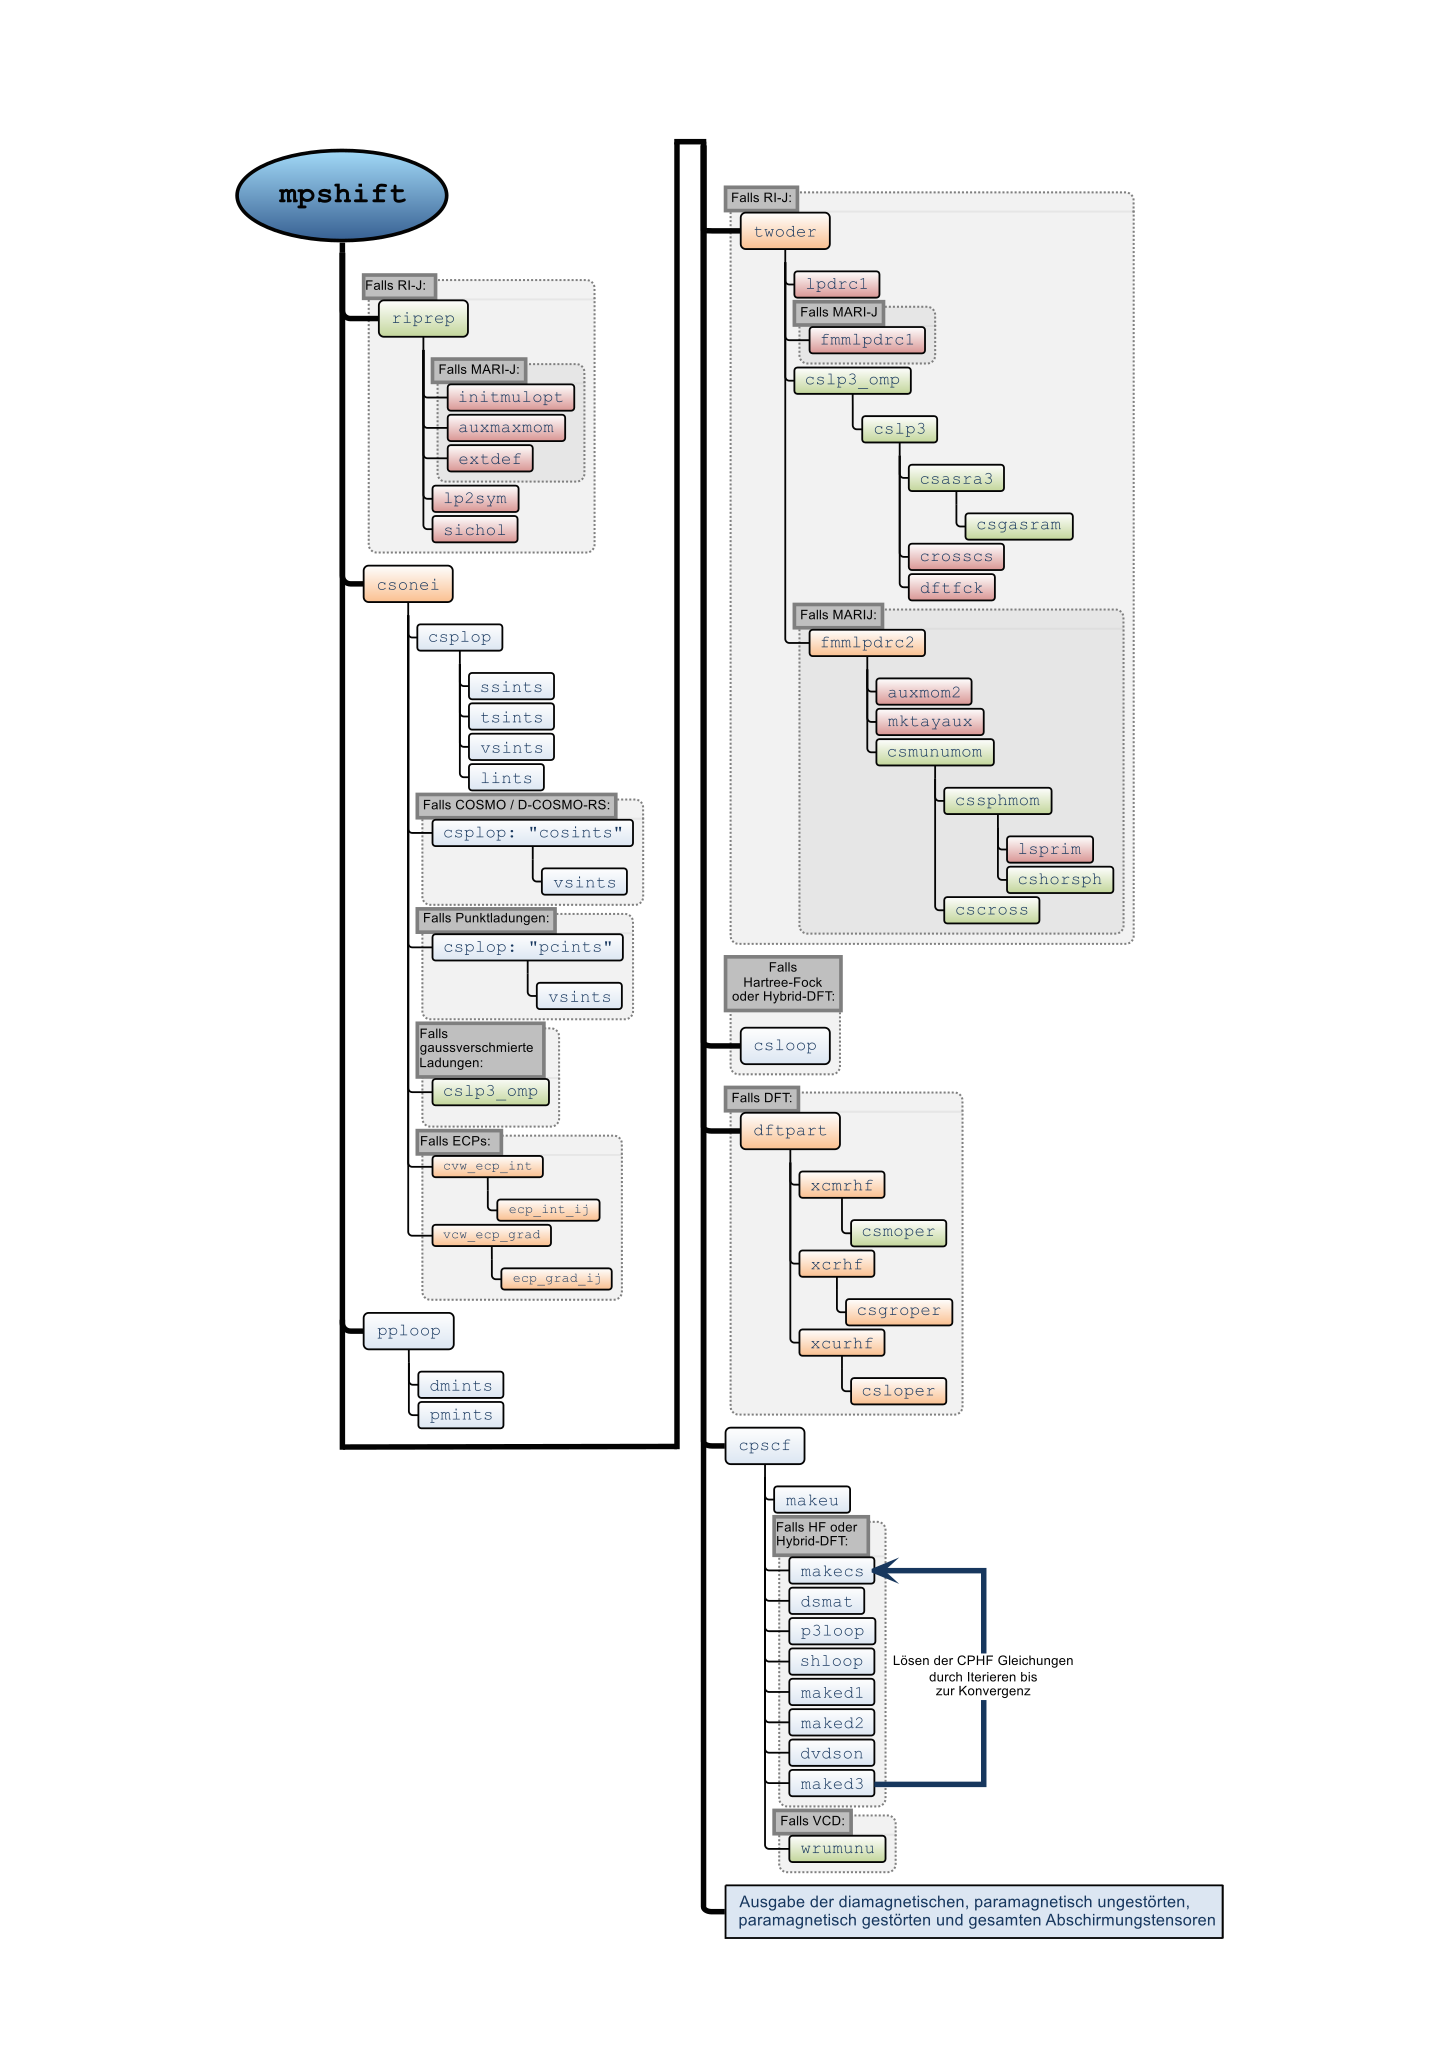
\includegraphics[width=0.9\textwidth]{mpshift_all}
	\captionsetup{figurewithin = chapter}
	\captionsetup{font=small, labelfont=bf}\caption[Neue schematische Programmstruktur des Moduls \texttt{mpshift}]{Schematische Programmstruktur des Moduls \texttt{mpshift} mit den wichtigsten Änderungen und Erweiterungen die im Rahmen der vorliegenden Arbeit durchgeführt wurden. Alte Routinen sind in blau, neue Routinen in grün, modifizierte Routinen in orange und unverändert aus anderen Modulen übertragene Routinen in rot dargestellt.}
\label{abb:neue_programmstruktur}
\end{figure}